\chapter{Matrix-Vector Product}

When we take the product of the matrix and the vector, 
it will result in a vector. The product is a contraction 
operation, which means that the matrix's dimension reduced from two to one.
To apply the contraction, then the length of one of the matrix dimensions 
must be the same as the vector's length.

Let the $A$ be the matrix with dimensions $m$ and $n$, 
and the length of the vector $x$ be $n$.

The resultant vector $y$ will have the dimension $m$.

\vspace*{0.5 cm}
$
A = 
\begin{bmatrix}
    a_{00}  & a_{01}    & \dots     & a_{0n}\\
    a_{10}  & a_{11}    & \dots     & a_{1n}\\
    \vdots  & \vdots    & \ddots    & \vdots\\
    a_{m0}  & a_{m1}    & \dots     & a_{mn}\\
\end{bmatrix}
, x =
\begin{bmatrix}
    x_0\\
    x_1\\
    \vdots\\
    x_n\\
\end{bmatrix}
$

\begin{equation}
    y = Ax + y
    \label{eq:mtv}
\end{equation}

$
Av = 
\begin{bmatrix}
    a_{00}  & a_{01}    & \dots     & a_{0n}\\
    a_{10}  & a_{11}    & \dots     & a_{1n}\\
    \vdots  & \vdots    & \ddots    & \vdots\\
    a_{m0}  & a_{m1}    & \dots     & a_{mn}\\
\end{bmatrix}
\begin{bmatrix}
    x_0\\
    x_1\\
    \vdots\\
    x_n\\
\end{bmatrix}
=
\begin{bmatrix}
    \sum_{i=0}^na_{0i}x_i\\
    \sum_{i=0}^na_{1i}x_i\\
    \vdots\\
    \sum_{i=0}^na_{mi}x_i\\
\end{bmatrix}
$

\vspace*{0.5 cm}
The vector times matrix can calculated by taking the transpose on the both sides.
\begin{align*}
    y^T &= (Ax + y)^T\\
    y^T &= (Ax)^T + y^T\\
    y^T &= x^TA^T + y^T\\
\end{align*}

The column-major and row-major layout for the vector in the memory 
is non-distinguishable. Hence, we can use this fact and we get $x = x^T$.
If $A$ is the column-major layout then $A^T$ is the row-major layout and vice-versa.

\begin{equation}
    y = xA^T + y
    \label{eq:vtm}
\end{equation}

\clearpage
\section{Calculating Number of Operations}

Using equation \ref{eq:mtv} or \ref{eq:vtm}, we fill the below table

\begin{table}[ht]
    \centering
    \begin{tabular}{|c|c|}
        \hline
        \textbf{Name} & \textbf{Number} \\
        \hline
        Multiplication & $m$ or $n$\\
        \hline
        Addition & $m-1$ or $n-1$ \\
        \hline
    \end{tabular}
\end{table}

Total Number of Operations $=$ (Number of Multiplication $+$ Number of Addition) $\times
\begin{cases}
    n \\
    m
\end{cases}
$

Total Number of Operations $= 
\begin{cases}
    n \times (m + m - 1)\\
    m  \times (n + n - 1)
\end{cases}
$

Total Number of Operations $= 
\begin{cases}
    n \times (2m - 1)\\
    m  \times (2n - 1)
\end{cases}
$

\section{Algorithm}
The matrix-vector product has two different algorithms: 
Column-Major and Row-Major. We need to handle two different 
layouts differently. 
The Row-Major has the most straightforward algorithm because 
the row elements lay contiguously in the memory, which improves 
the cache locality compared against Column-Major, where the row 
elements placed with a specific stride and hinder the cache locality.

\subsection{Column-Major}

\begin{algorithm}[H]
    \SetAlgoLined
    \SetKwFunction{SIMDFnFirst}{$simd\_loop_0$}
    \SetKwFunction{SIMDFnSecond}{$simd\_loop_1$}
    \SetKwProg{Fn}{Function}{:}{end}

    \tcp{$c$ is the pointer to the output vector}
    \tcp{$a$ is the pointer to the input matrix}
    \tcp{$b$ is the pointer to the input vector}
    \tcp{$k$ is the contracting dimension}
    \tcp{$m$ is the non-contracting dimension}
    \tcp{$w$ is the leading dimension of the matrix}
    \Fn{\SIMDFnFirst($c$, $a$, $b$, $k$, $w$)}{
        \openmp{simd reduction$(+:c[0:m_r])$}
        \For{\assign{i}{0} \KwTo $k$ \KwBy $1$}{
            \For{\assign{j}{0} \KwTo $m_r$ \KwBy $1$}{
                \assignln{c[i]}{c[i] + a[j + i * w] * b[i]}
            }
        }
    }
    \Fn{\SIMDFnSecond($c$, $a$, $b$, $m$, $k$, $w$)}{
        \openmp{simd reduction$(+:c[0:m_r])$}
        \For{\assign{j}{0} \KwTo $m$ \KwBy $1$}{
            \For{\assign{i}{0} \KwTo $k$ \KwBy $1$}{
                \assignln{c[i]}{c[i] + a[j + i * w] * b[i]}
            }
        }
    }
    \caption{Matrix-Vector Product SIMD Function}
\end{algorithm}

\begin{algorithm}[H]
    \SetAlgoLined
    \KwIn{$c$, $a$, $n_a$, $w_a$, $b$, $n_b$, $max\_threads$}
    \tcp{$c$ is the pointer to the output vector}
    \tcp{$a$ and $b$ are pointer to the matrix}
    \tcp{$b$ are pointer to the vector}
    \tcp{$n_a$ is the pointer to the extents of the matrix $a$}
    \tcp{$w_a$ is the pointer to the strides of the matrix $a$}
    \tcp{$n_b$ is the size of the vector $b$}
    \tcp{$max\_threads$ is the user provided thread count}

    \Begin{
        $omp\_set\_num\_threads(max\_threads)$
        
        \tcp{$m_r$ is the micro-tile}
        
        \assignln{M}{n_a[0]}
        \assignln{N}{n_a[1]}
        \assignln{lda}{max(w_a[0],w_a[1])}
        
        \tcp{$N_b$ macro-tile for contracting dimension}
        \tcp{$M_b$ macro-tile for non-contracting dimension and should be the multiple of $m_r$}

        \openmp{parallel for}
        \For{\assign{i}{0} \KwTo $M$ \KwBy $M_b$}{
            \assignln{i_b}{min(M-i,\ m_b)}
            \assignln{a_i}{a + i \times w_a[0]}
            \assignln{b_i}{b}
            \assignln{c_i}{c + i}
            \For{\assign{k}{0} \KwTo $N$ \KwBy $N_b$}{
                \assignln{k_b}{min(N-k,\ k_b)}
                \assignln{a_k}{a_i + k \times w_a[1]}
                \assignln{b_k}{b_i + k}
                \assignln{c_k}{c_i}
                \assignln{M_{iter}}{\lfloor \frac{i_b}{m_r} \rfloor}
                \assignln{M_{rem}}{i_b - (M_{iter} \times m_r)}
                $simd\_loop_1(c_k, a_k, b_k, M_{rem}, k_b, lda)$
                
                \assignln{a_k}{a_k + M_{rem} \times w_a[0]}
                \assignln{c_k}{c_k + M_{rem}}
                
                \For{\assign{ii}{0} \KwTo $M_{iter}$ \KwBy $1$}{
                    \assignln{a_p}{a_i + ii \times m_r \times w_a[1]}
                    \assignln{b_p}{b_i + ii \times m_r}
                    \assignln{c_p}{c_i}
                    $simd\_loop_0(c_p, a_p, b_p, k_b, lda)$
                }
            }
        }
    }

    \caption{Col-Major Matrix-Vector Product}
\end{algorithm}

The Column-Major product is quite tricky and complicated if 
we cannot control the instruction set. 
The row elements are $x$ strides away from each other and 
paralyse the cache predictor or cache locality. 
The cache predictor brings the cache line size elements 
from memory, which are place contiguously. 
Each element in the result vector is the product of the 
matrix's row vector and the whole vector. 

The algorithm for the matrix times vector is similar to Blis' algorithm, 
which describes the inner working of the matrix times matrix in the paper \cite{BLIS}. 
However, there are a few differences which are as following:
\begin{itemize}
    \item We do not pack the matrix.
    \item We do not use the micro-tile of the contracting dimension.
    \item We use two levels of cache.
\end{itemize}

We do not pack because of the time complexity of the packing and the matrix times vector 
complexity. The copying and operation time complexity is $O(N^2)$, but the copying overwhelms 
the operation and degrades the performance.

\begin{figure}[htb]
    \centering
    \caption{Column-Major Matrix-Vector Block Diagram}
    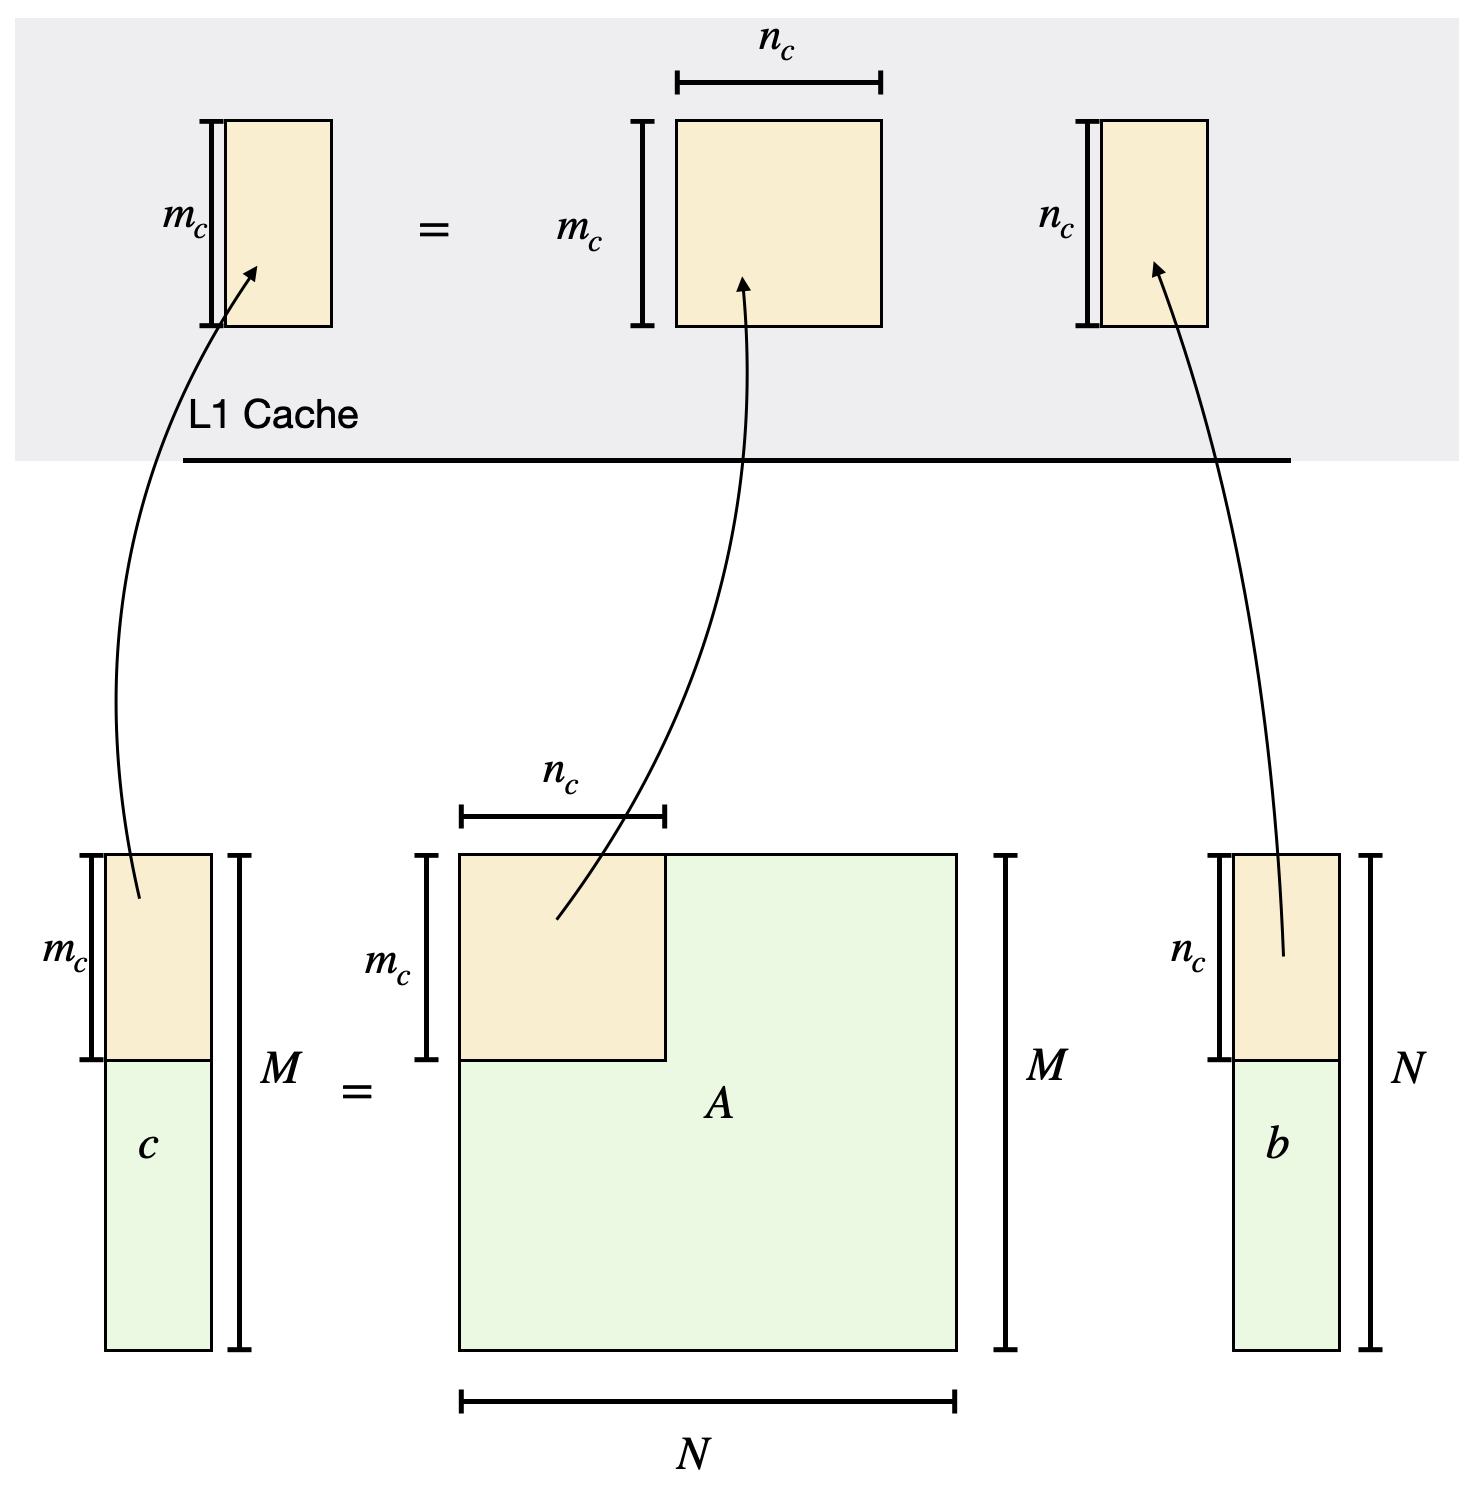
\includegraphics[width=10cm]{../assets/mtv/col_major/block_diagram.png} %
    \label{fig:mtv_col_block_diagram}
\end{figure}

Let macro-tile of the matrix $A$ be $A_c$, 
macro-tile of the vector $b$ be $b_c$, 
micro-tile of the input matrix be $A_r$, 
micro-tile of the input vector be $b_r$, and 
micro-tile of the output vector be $c_r$.

To maximize the performance, we try to maximize the 
reuse factors—the innermost micro-tiles, $c_r$, calculated 
using the equation defined in the paper \cite{BLIS}. Afterwards, 
we go from cache $L_1$ to cache $L_2$, figuring 
out the size of the macro-tiles. Then, the macro-tile, 
$A_c$, is put in the cache $L_2$ to maximize the reuse 
factor and macro-tile, $b_c$ kept in the cache $L_1$. 
Finally, we keep the macro-tile $b_c$ in the cache $L_1$ 
because it avoids bringing the micro-tile $c_r$ multiple 
times and increasing the reuse of $c_r$, which avoids 
polluting the cache or evicting the following tile 
and increases the probability of the next tile to 
present inside the $L_1$ cache. 

For finding the $m_r$ and $n_r$ refer to the section \ref{sec:mr_nr_calculation}, where
we went into much more detail.

\subsection{Macro-Tiles $n_c$ and $m_c$}

To find $n_c$, we have to focus on the cache $L_1$. 
For the $b_c$ not to be evicted from the $L_1$, we 
want $A_{r_{prev}}$ to replace $A_{r_{next}}$ rather than replacing $b_c$ 
because we assume the cache replacing algorithm 
to be LRU, and the old cache line is replaced by the 
new cache line. Therefore, we have to use $A_r$ to 
find the size $n_c$ and consider $c_r$, which will go 
through the caches to load inside the register. 
When $c_r$ loads, then it will replace the tiles that 
we put inside the caches in order to maximize the 
reuse factor and needs a whole one cache line reserved for it.

\begin{equation}
    A_r = S_{data} m_r n_c = C_{A_r}N_{L_1}C_{L_1}
    \label{eq:mtv_ar}
\end{equation}

\begin{equation}
    b_c = S_{data} n_c = C_{b_c}N_{L_1}C_{L_1}
    \label{eq:mtv_bc}
\end{equation}

Where $C_{A_r}$ is a integral factor and denotes the number of cache-line taken by the
micro-tile, $A_r$.

\begin{equation}
    C_{A_r} + C_{b_c} \leq W_{L_1} - 1
    \label{eq:mtv_W}
\end{equation}

Dividing the equation \ref{eq:mtv_ar} and \ref{eq:mtv_bc}, we get
\begin{align*}
    m_r &= \frac{C_{A_r}}{C_{b_c}}\\
    C_{b_c} &= \frac{C_{A_r}}{m_r}
\end{align*}

Substituting in \ref{eq:mtv_W}, we get

\[
    C_{A_r}(1 + \frac{1}{m_r}) \leq W_{L_1} - 1
\]

\[
    C_{A_r} = \lceil \frac{W_{L_1} - 1}{1 + \frac{1}{m_r}} \rceil
\]

But $1 + \frac{1}{m_r} \approx 1$ because $\frac{1}{m_r}$ tends toward zero for large value of $m_r$ 
and we can ignore the denominator.

\begin{equation}
    C_{A_r} = W - 1
    \label{eq:mtv_car}
\end{equation}

\begin{align*}
    n_c = \frac{ (W_{L_1} - 1) N_{L_1}C_{L_1} }{S_{data} m_r }
\end{align*}

Similarly, we can calculate the $m_c$, and we get

\begin{align*}
    m_c = \frac{ (W_{L_2} - 1) N_{L_2}C_{L_2} }{S_{data} n_c }
\end{align*}

But, there is a one difference here we need to worry about the $A_c$ and for others 
we can reserve one cache-line for them pass through.

\clearpage
\subsection{Row-Major}

\begin{algorithm}[H]
    \SetAlgoLined
    \SetKwFunction{SIMDFn}{$simd\_loop$}
    \SetKwProg{Fn}{Function}{:}{end}

    \tcp{$a$ is the pointer to the input matrix}
    \tcp{$b$ is the pointer to the input vector}
    \tcp{$n_b$ is the block of the output vector}
    \Fn{\SIMDFn($a$, $b$, $n_b$)}{
        \assignln{sum}{0}
        \openmp{simd}
        \For{\assign{i}{0} \KwTo $n_b$ \KwBy $1$}{
            \assignln{sum}{sum + a[i] \times b[i]}
        }
        \KwRet{sum}
    }
    \caption{Matrix-Vector Product SIMD Function}
\end{algorithm}

\begin{algorithm}[H]
    \SetAlgoLined
    \KwIn{$c$, $a$, $n_a$, $w_a$, $b$, $n_b$, $max\_threads$}
    \tcp{$c$ is the pointer to the output vector}
    \tcp{$a$ and $b$ are pointer to the matrix}
    \tcp{$b$ are pointer to the vector}
    \tcp{$n_a$ is the size of the column of the matrix $a$}
    \tcp{$w_a$ is the leading dimension of the matrix $a$}
    \tcp{$n_b$ is the size of the vector $b$}
    \tcp{$max\_threads$ is the user provided thread count}

    \Begin{
        $omp\_set\_num\_threads(max\_threads)$

        \assignln{ai}{a}
        \assignln{bi}{b}
        \assignln{ci}{c}
        
        \openmp{parallel for schedule(static)}
        \For{\assign{i}{0} \KwTo $n_a$ \KwBy $1$}{
            \assignln{aj}{ai + i * w_a}
            \assignln{bj}{bi}
            \assignln{cj}{ci + i}
            \assignln{cj}{simd\_loop(aj,bj,n_b)}
        }
    }

    \caption{Row-Major Matrix-Vector Product}
\end{algorithm}

The Row-Major product is the simplest one because the row elements 
are contiguous in memory; therefore, each thread assigned to each 
row vector, and they are responsible for each element of the output 
vector. The distribution of the row-vector to the threads simplifies 
the problem to the vector-vector inner product. The inner product of 
the row-vector and the input vector gives an element of the output vector.

\begin{figure}[htb]
    \centering
    \caption{Row-Major Matrix-Vector Block Diagram}
    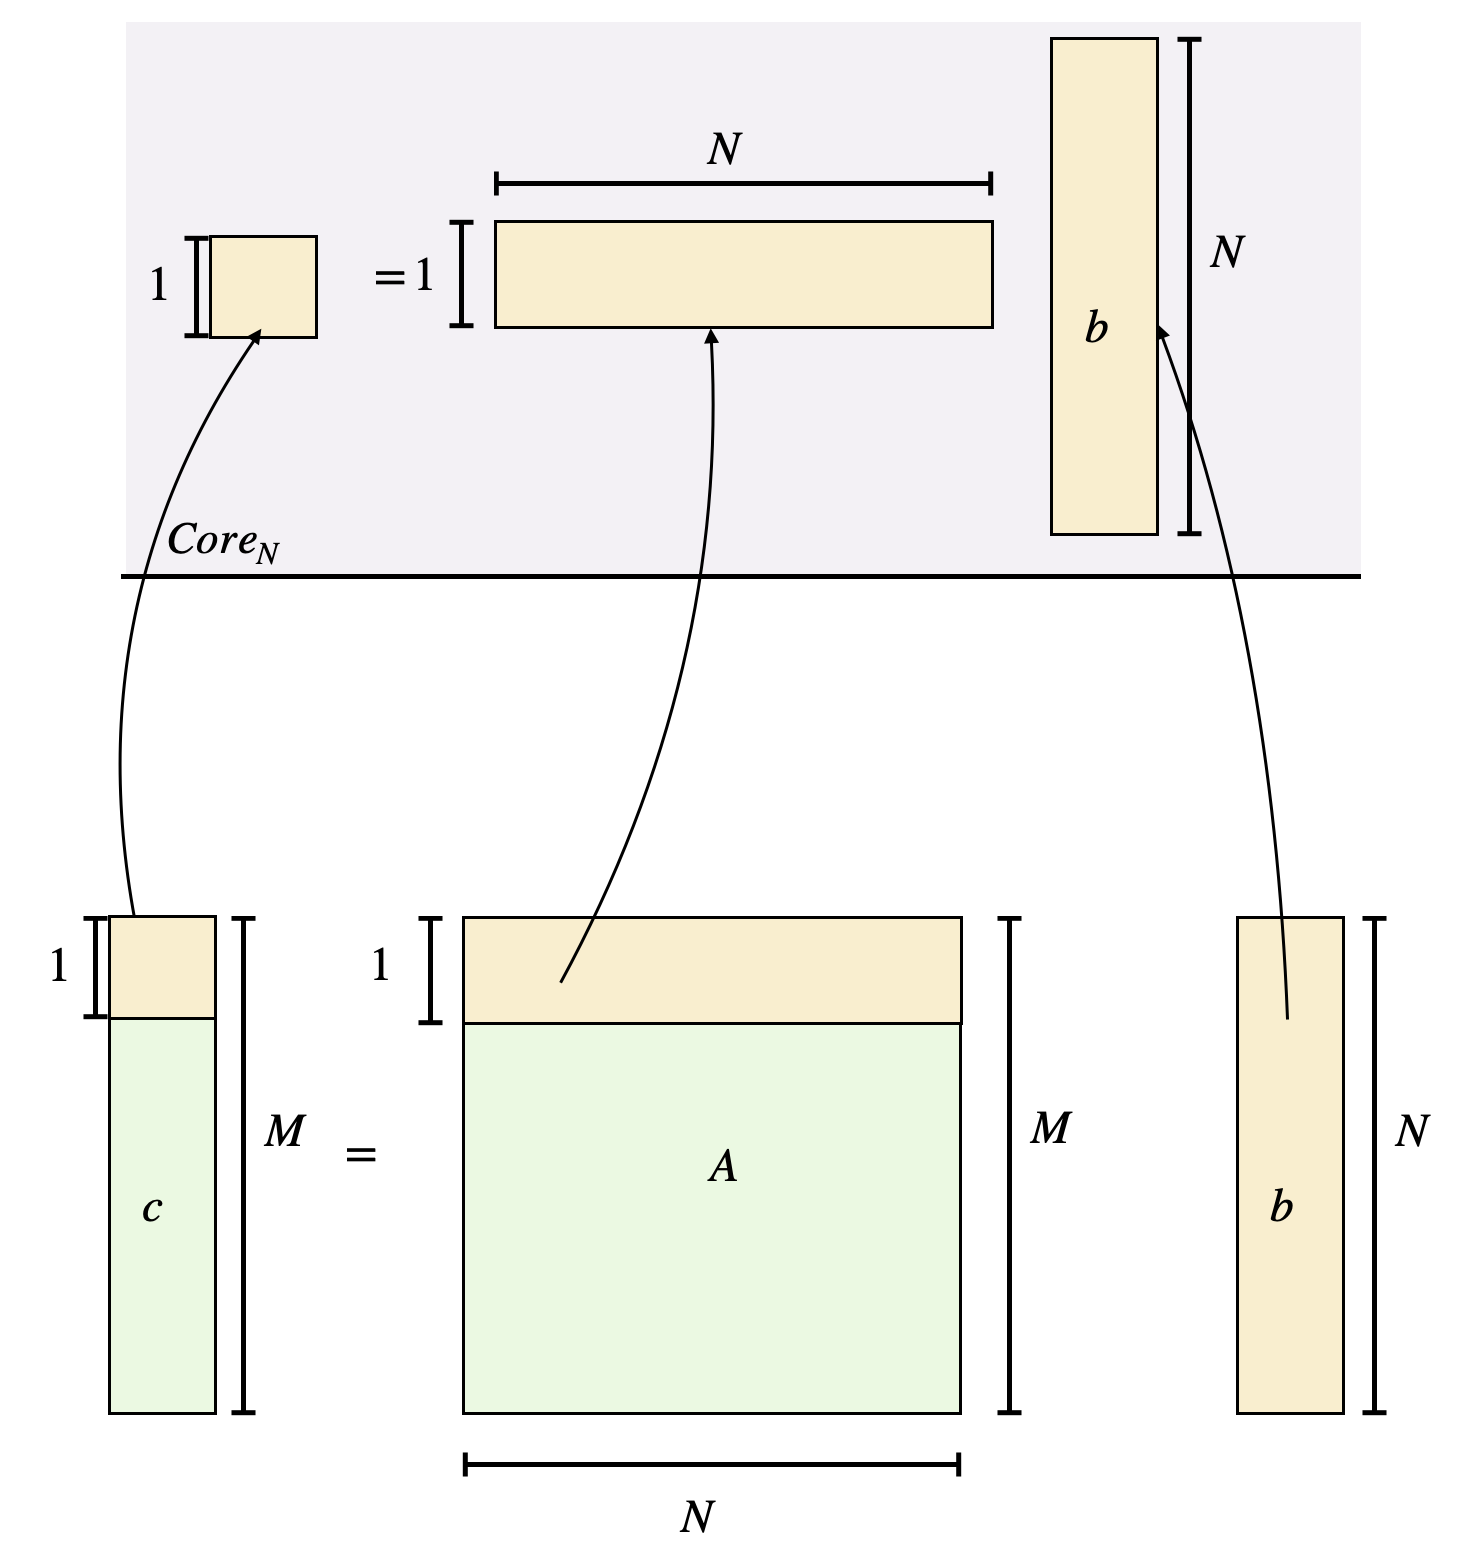
\includegraphics[width=15cm]{../assets/mtv/row_major/block_diagram.png} %
\end{figure}

\clearpage
\section{Performance Plots and Speedup Summary For Column-Major}

\begin{figure}[htb]
    \centering
    \caption*{Performance measurements of ?gemv implementations}
    \subfloat[\centering Single-Precision]{{\includegraphics[width=8cm]{../assets/mtv/col_major/float_GflopsVsSize.png} }}%
    \label{fig:mtv_col_Sgflop220}
    \qquad
    \subfloat[\centering Double-Precision]{{\includegraphics[width=8cm]{../assets/mtv/col_major/double_GflopsVsSize.png} }}%
    \label{fig:mtv_col_Dgflop220}
\end{figure}

\begin{figure}[htb]
    \centering
    \caption*{Sorted performance measurements of ?gemv implementations}
    \subfloat[\centering Single-Precision]{{\includegraphics[width=8cm]{../assets/mtv/col_major/float_GflopsVsSize_per.png} }}%
    \label{fig:mtv_col_Sgflop_per220}
    \qquad
    \subfloat[\centering Double-Precision]{{\includegraphics[width=8cm]{../assets/mtv/col_major/double_GflopsVsSize_per.png} }}%
    \label{fig:mtv_col_Dgflop_per220}
\end{figure}

\begin{figure}[htb]
    \centering
    \caption*{Comparison of the Boost.uBLAS.Tensor ?gemv implementation}
    \subfloat[\centering Single-Precision]{{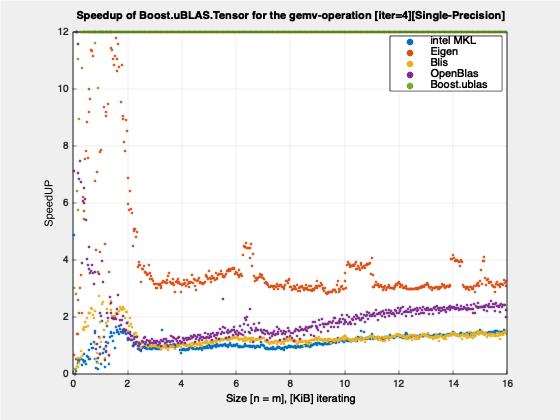
\includegraphics[width=8cm]{../assets/mtv/col_major/float_Speedup.png} }}%
    \label{fig:mtv_col_Sspeedup220}
    \qquad
    \subfloat[\centering Double-Precision]{{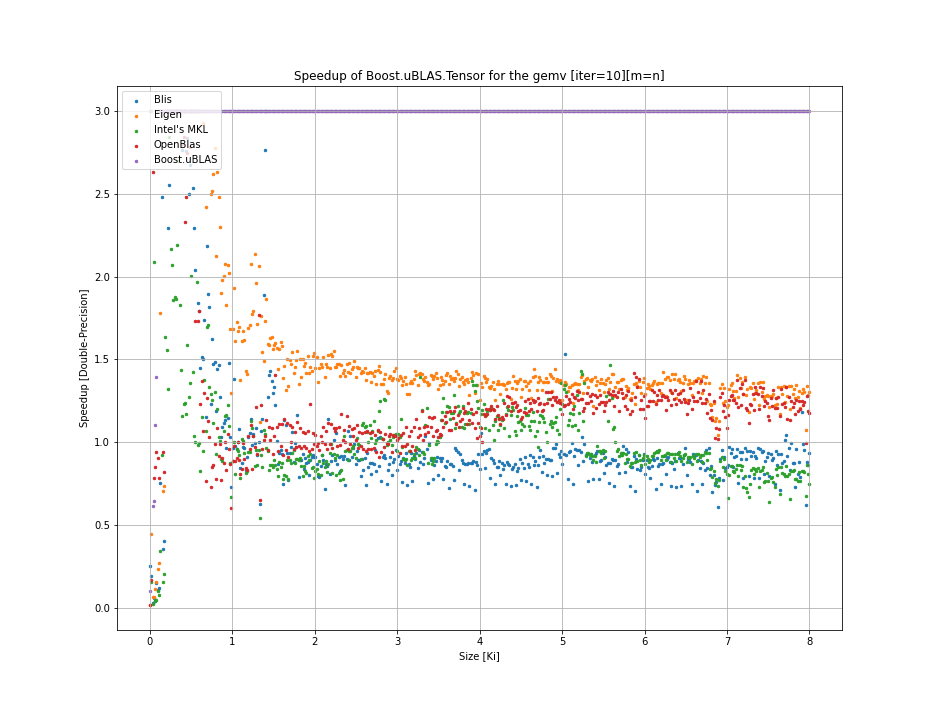
\includegraphics[width=8cm]{../assets/mtv/col_major/double_Speedup.png} }}%
    \label{fig:mtv_col_Dspeedup220}
\end{figure}

\begin{figure}[htb]
    \centering
    \caption*{Comparison of the Boost.uBLAS.Tensor ?gemv implementation [semilogy]}
    \subfloat[\centering Single-Precision]{{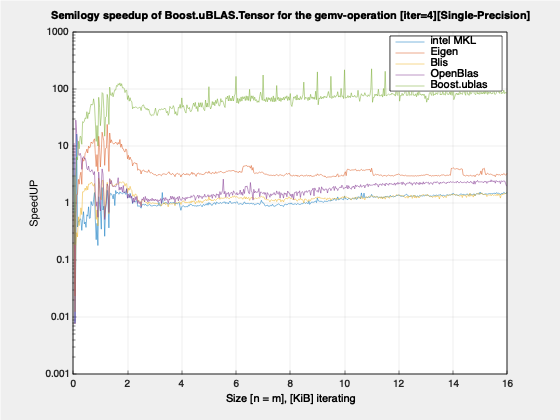
\includegraphics[width=8cm]{../assets/mtv/col_major/float_Speedup_log10.png} }}%
    \label{fig:mtv_col_Sspeedup_log10220}
    \qquad
    \subfloat[\centering Double-Precision]{{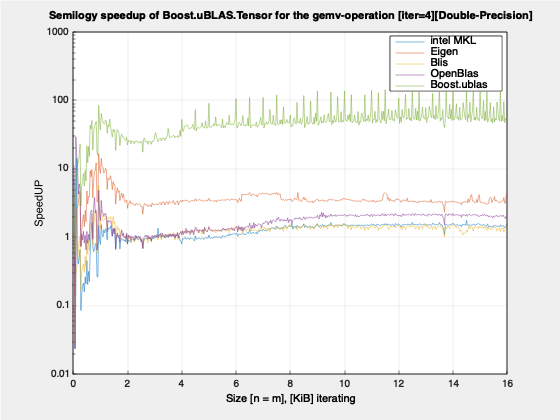
\includegraphics[width=8cm]{../assets/mtv/col_major/double_Speedup_log10.png} }}%
    \label{fig:mtv_col_Dspeedup_log10220}
\end{figure}

\begin{figure}[htb]
    \centering
    \caption*{Comparison of the Boost.uBLAS.Tensor ?gemv implementation [sorted]}
    \subfloat[\centering Single-Precision]{{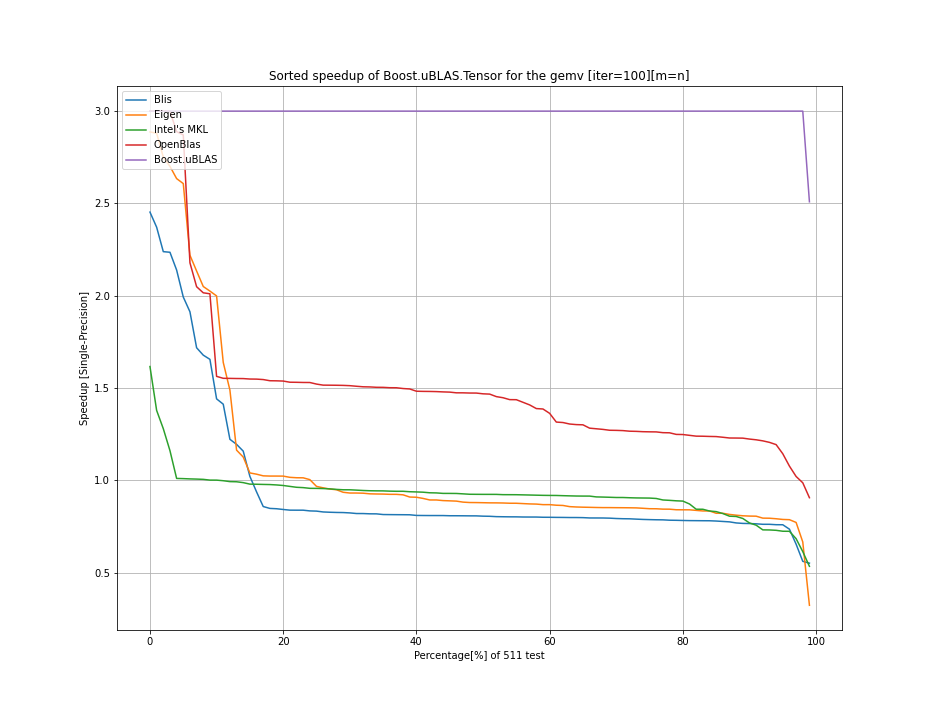
\includegraphics[width=8cm]{../assets/mtv/col_major/float_Speedup_per.png} }}%
    \label{fig:mtv_col_Sspeedup_per220}
    \qquad
    \subfloat[\centering Double-Precision]{{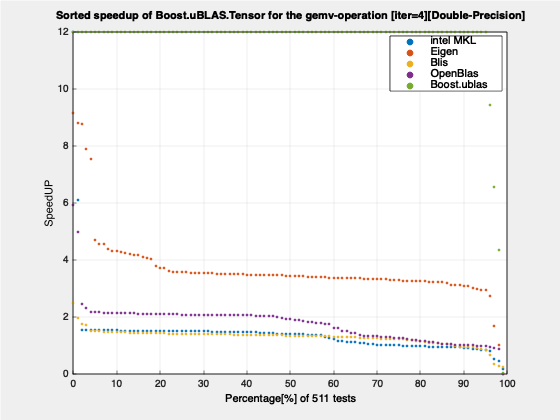
\includegraphics[width=8cm]{../assets/mtv/col_major/double_Speedup_per.png} }}%
    \label{fig:mtv_col_Dspeedup_per220}
\end{figure}

\begin{table}[ht]
    \centering
    \caption{Speedup Summary For Single-Precision}
    \begin{tabular}{|l|c|c|}
        \hline
        \textbf{Implementation} & \textbf{Speedup $\geq$ 1 [\%]} & \textbf{Speedup $\geq$ 2 [\%]}\\
        \hline
        Boost.uBLAS & $99$ & $99$ \\
        \hline
        OpenBLAS    & $97$ & $9$ \\
        \hline
        Eigen       & $24$ & $9$ \\
        \hline
        Blis        & $98$ & $98$ \\
        \hline
        Intel's MKL & $10$ & $0$ \\
        \hline
    \end{tabular}
    
    \begin{tabular}{|l|c|c|}
        \hline
        \textbf{Implementation} & \textbf{Speed-down $\geq$ 1 [\%]} & \textbf{Speed-down $\geq$ 2 [\%]}\\
        \hline
        Boost.uBLAS & $0$ & $0$ \\
        \hline
        OpenBLAS    & $3$ & $0$ \\
        \hline
        Eigen       & $76$ & $0$ \\
        \hline
        Blis        & $86$ & $0$ \\
        \hline
        Intel's MKL & $91$ & $0$ \\
        \hline
    \end{tabular}
    
    \vspace*{1 cm}

    \centering
    \caption{Speedup Summary For Double-Precision}
    \begin{tabular}{|l|c|c|}
        \hline
        \textbf{Implementation} & \textbf{Speedup $\geq$ 1 [\%]} & \textbf{Speedup $\geq$ 2 [\%]}\\
        \hline
        Boost.uBLAS & $99$ & $98$ \\
        \hline
        OpenBLAS    & $89$ & $4$ \\
        \hline
        Eigen       & $98$ & $8$ \\
        \hline
        Blis        & $14$ & $3$ \\
        \hline
        Intel's MKL & $40$ & $0$ \\
        \hline
    \end{tabular}
    
    \begin{tabular}{|l|c|c|}
        \hline
        \textbf{Implementation} & \textbf{Speed-down $\geq$ 1 [\%]} & \textbf{Speed-down $\geq$ 2 [\%]}\\
        \hline
        Boost.uBLAS & $0$ & $0$ \\
        \hline
        OpenBLAS    & $9$ & $0$ \\
        \hline
        Eigen       & $1$ & $1$ \\
        \hline
        Blis        & $86$ & $1$ \\
        \hline
        Intel's MKL & $60$ & $2$ \\
        \hline
    \end{tabular}
\end{table}

\clearpage
\section{Performance Metrics For Column-Major}

\subsection*{Range[Start: $32$, End: $16382$, Step: $32$]}

\begin{table}[ht]
    \centering
    \caption{GFLOPS For Single-Precision}
    \begin{tabular}{|l|c|c|}
        \hline
        \textbf{Implementation} & \textbf{Max} & \textbf{Average}\\
        \hline
        Boost.uBLAS.Tensor  & $107.22$& $14.4079$ \\
        \hline
        Boost.uBLAS         & $1.02227$& $0.271$ \\
        \hline
        Intel's MKL         & $87.6178$& $15.789$ \\
        \hline
        OpenBLAS            & $44.5053$& $8.4120$ \\
        \hline
        Blis                & $36.8396$& $12.9113$ \\
        \hline
        Eigen               & $32.9823$& $11.4342$ \\
        \hline
    \end{tabular}

    \vspace*{1 cm}

    \centering
    \caption{GFLOPS For Double-Precision}
    \begin{tabular}{|l|c|c|}
        \hline
        \textbf{Implementation} & \textbf{Max} & \textbf{Average}\\
        \hline
        Boost.uBLAS.Tensor  & $52.144$ & $6.2511$ \\
        \hline
        Boost.uBLAS         & $0.6601$ & $0.1828$ \\
        \hline
        Intel's MKL         & $33.6268$ & $6.0042$ \\
        \hline
        OpenBLAS            & $16.1558$ & $4.4325$ \\
        \hline
        Blis                & $17.4944$ & $5.41638$ \\
        \hline
        Eigen               & $6.30737$ & $3.26405$ \\
        \hline
    \end{tabular}
\end{table}

\begin{table}[ht]
    \centering
    \caption{Utilization[\%] For Single-Precision}
    \begin{tabular}{|l|c|c|}
        \hline
        \textbf{Implementation} & \textbf{Max} & \textbf{Average}\\
        \hline
        Boost.uBLAS.Tensor  & $12.730$& $1.710$ \\
        \hline
        Boost.uBLAS         & $0.121$& $0.032$ \\
        \hline
        Intel's MKL         & $10.402$& $1.874$ \\
        \hline
        OpenBLAS            & $5.284$& $0.998$ \\
        \hline
        Blis                & $4.374$& $1.532$ \\
        \hline
        Eigen               & $3.916$& $1.357$ \\
        \hline
    \end{tabular}

    \vspace*{1 cm}

    \centering
    \caption{Utilization[\%] For Double-Precision}
    \begin{tabular}{|l|c|c|}
        \hline
        \textbf{Implementation} & \textbf{Max} & \textbf{Average}\\
        \hline
        Boost.uBLAS.Tensor  & $12.382$ & $1.484$ \\
        \hline
        Boost.uBLAS         & $0.156$ & $0.043$ \\
        \hline
        Intel's MKL         & $7.985$ & $1.425$ \\
        \hline
        OpenBLAS            & $3.836$ & $1.052$ \\
        \hline
        Blis                & $4.154$ & $1.286$ \\
        \hline
        Eigen               & $1.497$ & $0.775$ \\
        \hline
    \end{tabular}
\end{table}

\begin{table}[ht]
    \centering
    \caption{Speedup(Boost.uBLAS.Tensor) For Single-Precision}
    \begin{tabular}{|l|c|c|}
        \hline
        \textbf{Implementation} & \textbf{Max} & \textbf{Average}\\
        \hline
        Boost.uBLAS         & $104.884$ & $53.092$ \\
        \hline
        Intel's MKL         & $1.2237$ & $0.9125$ \\
        \hline
        OpenBLAS            & $2.4091$ & $1.7127$ \\
        \hline
        Blis                & $2.9104$ & $1.11590$ \\
        \hline
        Eigen               & $3.2508$ & $1.26006$ \\
        \hline
    \end{tabular}

    \vspace*{1 cm}

    \centering
    \caption{Speedup(Boost.uBLAS.Tensor) For Double-Precision}
    \begin{tabular}{|l|c|c|}
        \hline
        \textbf{Implementation} & \textbf{Max} & \textbf{Average}\\
        \hline
        Boost.uBLAS         & $78.9937$ & $34.195$ \\
        \hline
        Intel's MKL         & $1.5506$ & $1.0411$ \\
        \hline
        OpenBLAS            & $3.2275$ & $1.4102$ \\
        \hline
        Blis                & $2.9806$ & $1.1541$ \\
        \hline
        Eigen               & $8.2671$ & $1.9151$ \\
        \hline
    \end{tabular}
\end{table}

\clearpage
\section{Performance Plots and Speedup Summary For Row-Major}

\begin{figure}[htb]
    \centering
    \caption*{Performance measurements of ?gemv implementations}
    \subfloat[\centering Single-Precision]{{\includegraphics[width=8cm]{../assets/mtv/row_major/float_GflopsVsSize.png} }}%
    \label{fig:mtv_row_Sgflop220}
    \qquad
    \subfloat[\centering Double-Precision]{{\includegraphics[width=8cm]{../assets/mtv/row_major/double_GflopsVsSize.png} }}%
    \label{fig:mtv_row_Dgflop220}
\end{figure}

\begin{figure}[htb]
    \centering
    \caption*{Sorted performance measurements of ?gemv implementations}
    \subfloat[\centering Single-Precision]{{\includegraphics[width=8cm]{../assets/mtv/row_major/float_GflopsVsSize_per.png} }}%
    \label{fig:mtv_row_Sgflop_per220}
    \qquad
    \subfloat[\centering Double-Precision]{{\includegraphics[width=8cm]{../assets/mtv/row_major/double_GflopsVsSize_per.png} }}%
    \label{fig:mtv_row_Dgflop_per220}
\end{figure}

\begin{figure}[htb]
    \centering
    \caption*{Comparison of the Boost.uBLAS.Tensor ?gemv implementation}
    \subfloat[\centering Single-Precision]{{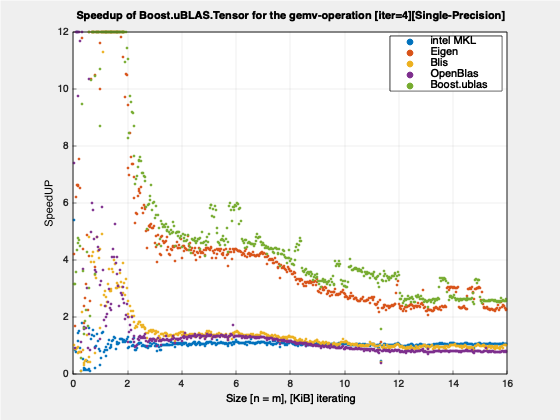
\includegraphics[width=8cm]{../assets/mtv/row_major/float_Speedup.png} }}%
    \label{fig:mtv_row_Sspeedup220}
    \qquad
    \subfloat[\centering Double-Precision]{{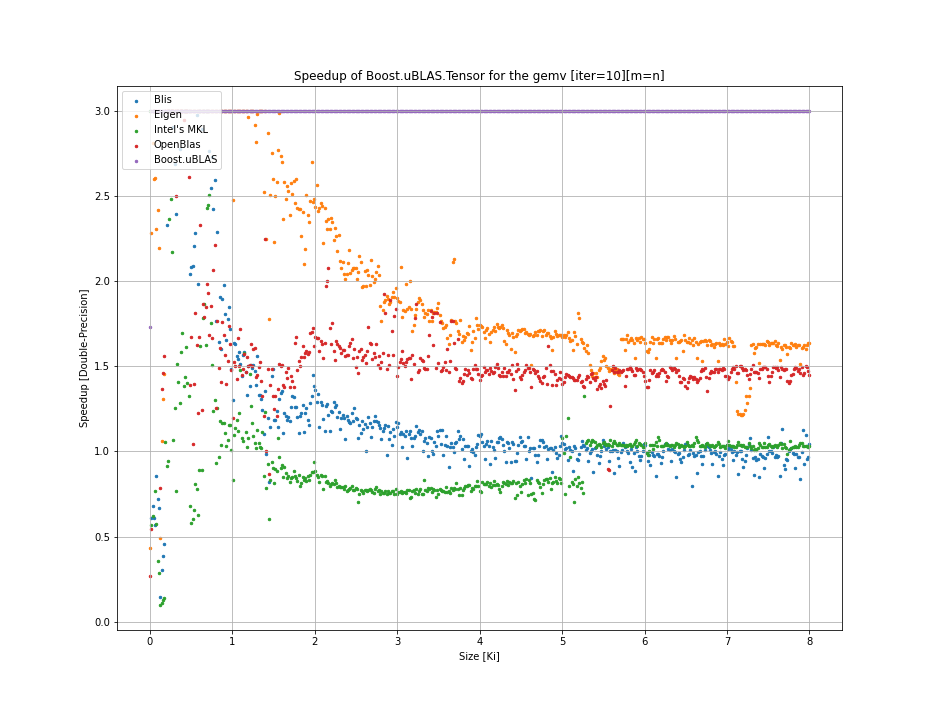
\includegraphics[width=8cm]{../assets/mtv/row_major/double_Speedup.png} }}%
    \label{fig:mtv_row_Dspeedup220}
\end{figure}

\begin{figure}[htb]
    \centering
    \caption*{Comparison of the Boost.uBLAS.Tensor ?gemv implementation [semilogy]}
    \subfloat[\centering Single-Precision]{{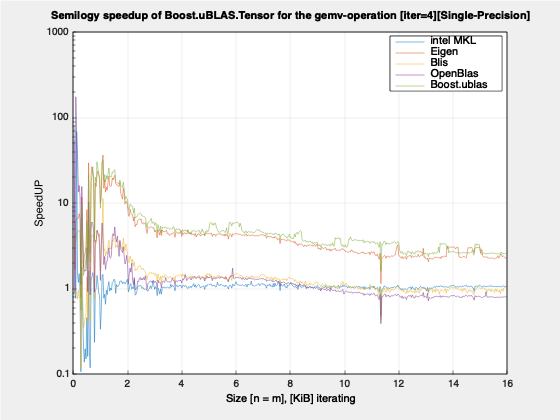
\includegraphics[width=8cm]{../assets/mtv/row_major/float_Speedup_log10.png} }}%
    \label{fig:mtv_row_Sspeedup_log10220}
    \qquad
    \subfloat[\centering Double-Precision]{{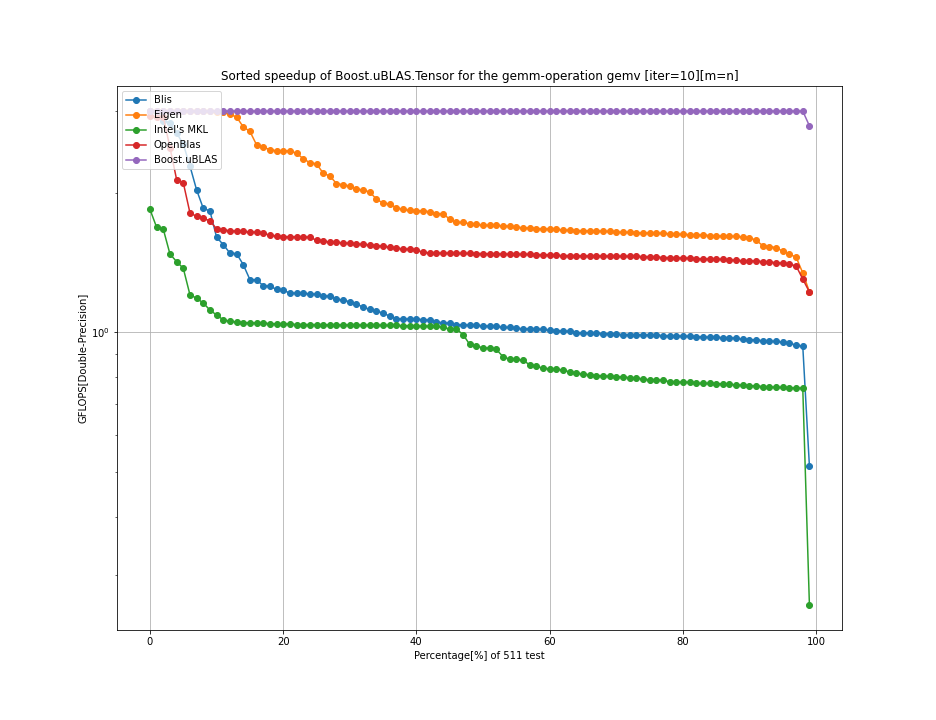
\includegraphics[width=8cm]{../assets/mtv/row_major/double_Speedup_log10.png} }}%
    \label{fig:mtv_row_Dspeedup_log10220}
\end{figure}

\begin{figure}[htb]
    \centering
    \caption*{Comparison of the Boost.uBLAS.Tensor ?gemv implementation [sorted]}
    \subfloat[\centering Single-Precision]{{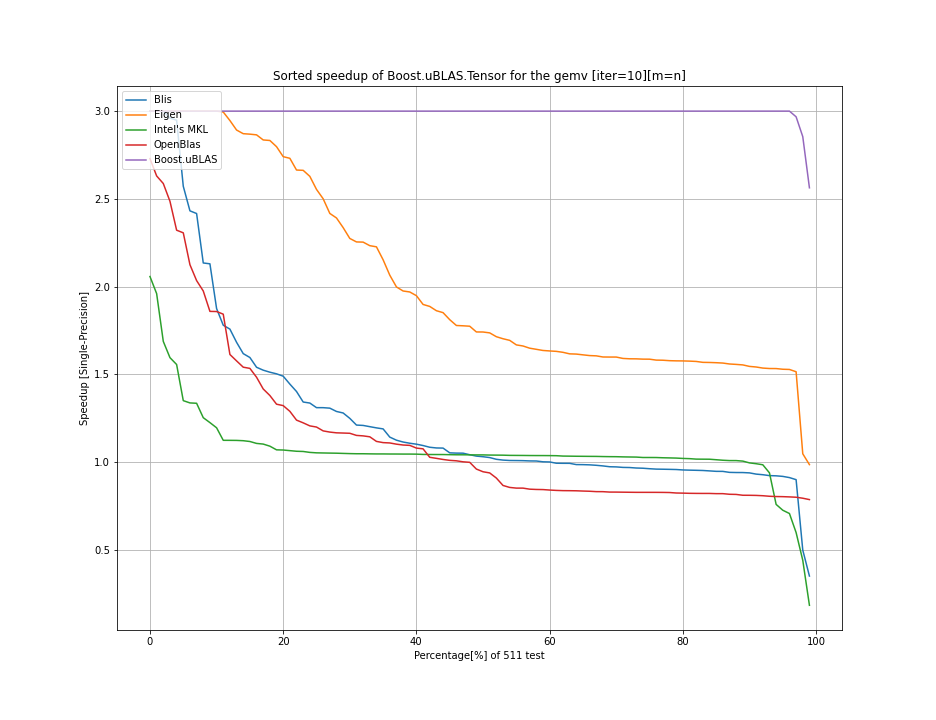
\includegraphics[width=8cm]{../assets/mtv/row_major/float_Speedup_per.png} }}%
    \label{fig:mtv_row_Sspeedup_per220}
    \qquad
    \subfloat[\centering Double-Precision]{{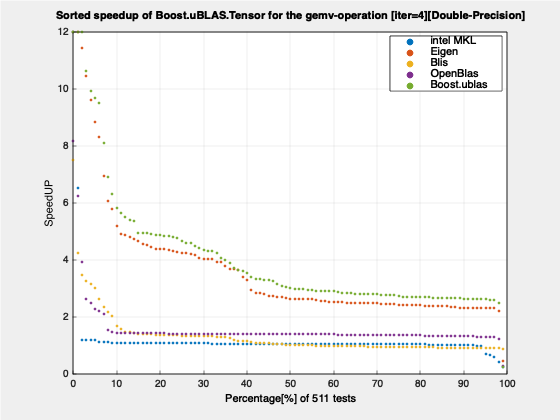
\includegraphics[width=8cm]{../assets/mtv/row_major/double_Speedup_per.png} }}%
    \label{fig:mtv_row_Dspeedup_per220}
\end{figure}

\begin{table}[ht]
    \centering
    \caption{Speedup Summary For Single-Precision}
    \begin{tabular}{|l|c|c|}
        \hline
        \textbf{Implementation} & \textbf{Speedup $\geq$ 1 [\%]} & \textbf{Speedup $\geq$ 2 [\%]}\\
        \hline
        Boost.uBLAS & $99$ & $99$ \\
        \hline
        OpenBLAS    & $47$ & $7$ \\
        \hline
        Eigen       & $98$ & $36$ \\
        \hline
        Blis        & $60$ & $9$ \\
        \hline
        Intel's MKL & $89$ & $0$ \\
        \hline
    \end{tabular}
    
    \begin{tabular}{|l|c|c|}
        \hline
        \textbf{Implementation} & \textbf{Speed-down $\geq$ 1 [\%]} & \textbf{Speed-down $\geq$ 2 [\%]}\\
        \hline
        Boost.uBLAS & $0$ & $0$ \\
        \hline
        OpenBLAS    & $54$ & $0$ \\
        \hline
        Eigen       & $2$ & $0$ \\
        \hline
        Blis        & $40$ & $1$ \\
        \hline
        Intel's MKL & $11$ & $1$ \\
        \hline
    \end{tabular}
    
    \vspace*{1 cm}

    \centering
    \caption{Speedup Summary For Double-Precision}
    \begin{tabular}{|l|c|c|}
        \hline
        \textbf{Implementation} & \textbf{Speedup $\geq$ 1 [\%]} & \textbf{Speedup $\geq$ 2 [\%]}\\
        \hline
        Boost.uBLAS & $99$ & $99$ \\
        \hline
        OpenBLAS    & $99$ & $5$ \\
        \hline
        Eigen       & $99$ & $33$ \\
        \hline
        Blis        & $63$ & $7$ \\
        \hline
        Intel's MKL & $46$ & $0$ \\
        \hline
    \end{tabular}
    
    \begin{tabular}{|l|c|c|}
        \hline
        \textbf{Implementation} & \textbf{Speed-down $\geq$ 1 [\%]} & \textbf{Speed-down $\geq$ 2 [\%]}\\
        \hline
        Boost.uBLAS & $0$ & $0$ \\
        \hline
        OpenBLAS    & $0$ & $0$ \\
        \hline
        Eigen       & $0$ & $0$ \\
        \hline
        Blis        & $36$ & $0$ \\
        \hline
        Intel's MKL & $53$ & $1$ \\
        \hline
    \end{tabular}
\end{table}

\clearpage
\section{Performance Metrics For Row-Major}

\subsection*{Range[Start: $32$, End: $16382$, Step: $32$]}

\begin{table}[ht]
    \centering
    \caption{GFLOPS For Single-Precision}
    \begin{tabular}{|l|c|c|}
        \hline
        \textbf{Implementation} & \textbf{Max} & \textbf{Average}\\
        \hline
        Boost.uBLAS.Tensor  & $130.099$& $17.812$ \\
        \hline
        Boost.uBLAS         & $1.7571$& $1.4884$ \\
        \hline
        Intel's MKL         & $87.2948$& $17.253$ \\
        \hline
        OpenBLAS            & $41.5645$& $13.712$ \\
        \hline
        Blis                & $42.0662$& $12.5435$ \\
        \hline
        Eigen               & $13.0251$& $6.5156$ \\
        \hline
    \end{tabular}

    \vspace*{1 cm}

    \centering
    \caption{GFLOPS For Double-Precision}
    \begin{tabular}{|l|c|c|}
        \hline
        \textbf{Implementation} & \textbf{Max} & \textbf{Average}\\
        \hline
        Boost.uBLAS.Tensor  & $77.7866$& $8.096$ \\
        \hline
        Boost.uBLAS         & $0.7437$& $0.666$ \\
        \hline
        Intel's MKL         & $49.3442$& $8.396$ \\
        \hline
        OpenBLAS            & $25.0278$& $4.4855$ \\
        \hline
        Blis                & $23.9759$& $5.7617$ \\
        \hline
        Eigen               & $5.57867$& $3.0228$ \\
        \hline
    \end{tabular}
\end{table}

\begin{table}[ht]
    \centering
    \caption{Utilization[\%] For Single-Precision}
    \begin{tabular}{|l|c|c|}
        \hline
        \textbf{Implementation} & \textbf{Max} & \textbf{Average}\\
        \hline
        Boost.uBLAS.Tensor  & $15.446$& $2.114$ \\
        \hline
        Boost.uBLAS         & $0.208$& $0.176$ \\
        \hline
        Intel's MKL         & $10.364$& $2.048$ \\
        \hline
        OpenBLAS            & $4.934$& $1.628$ \\
        \hline
        Blis                & $4.994$& $1.489$ \\
        \hline
        Eigen               & $1.546$& $0.773$ \\
        \hline
    \end{tabular}

    \vspace*{1 cm}

    \centering
    \caption{Utilization[\%] For Double-Precision}
    \begin{tabular}{|l|c|c|}
        \hline
        \textbf{Implementation} & \textbf{Max} & \textbf{Average}\\
        \hline
        Boost.uBLAS.Tensor  & $18.471$& $1.922$ \\
        \hline
        Boost.uBLAS         & $0.176$& $0.158$ \\
        \hline
        Intel's MKL         & $11.717$& $1.993$ \\
        \hline
        OpenBLAS            & $5.943$& $1.065$ \\
        \hline
        Blis                & $5.693$& $1.368$ \\
        \hline
        Eigen               & $1.324$& $0.717$ \\
        \hline
    \end{tabular}
\end{table}

\begin{table}[ht]
    \centering
    \caption{Speedup(Boost.uBLAS.Tensor) For Single-Precision}
    \begin{tabular}{|l|c|c|}
        \hline
        \textbf{Implementation} & \textbf{Max} & \textbf{Average}\\
        \hline
        Boost.uBLAS         & $74.041$& $11.9676$ \\
        \hline
        Intel's MKL         & $1.4903$& $1.032$ \\
        \hline
        OpenBLAS            & $3.1300$& $1.2990$ \\
        \hline
        Blis                & $3.0927$& $1.4200$ \\
        \hline
        Eigen               & $9.9883$& $2.7338$ \\
        \hline
    \end{tabular}

    \vspace*{1 cm}

    \centering
    \caption{Speedup(Boost.uBLAS.Tensor) For Double-Precision}
    \begin{tabular}{|l|c|c|}
        \hline
        \textbf{Implementation} & \textbf{Max} & \textbf{Average}\\
        \hline
        Boost.uBLAS         & $104.589$& $12.1426$ \\
        \hline
        Intel's MKL         & $1.5764$& $0.96423$ \\
        \hline
        OpenBLAS            & $3.108$& $1.8049$ \\
        \hline
        Blis                & $3.2443$& $1.40512$ \\
        \hline
        Eigen               & $13.9435$& $2.6783$ \\
        \hline
    \end{tabular}
\end{table}